%%%%%%%%%%%%%%%%%%%%%%%%%%%%%%%%%%%%%%%%%
% baposter Landscape Poster
% LaTeX Template
% Version 1.0 (11/06/13)
%
% baposter Class Created by:
% Brian Amberg (baposter@brian-amberg.de)
%
% This template has been downloaded from:
% http://www.LaTeXTemplates.com
%
% License:
% CC BY-NC-SA 3.0 (http://creativecommons.org/licenses/by-nc-sa/3.0/)
%
%%%%%%%%%%%%%%%%%%%%%%%%%%%%%%%%%%%%%%%%%

%----------------------------------------------------------------------------------------
%	PACKAGES AND OTHER DOCUMENT CONFIGURATIONS
%----------------------------------------------------------------------------------------

\documentclass[landscape,a0paper,fontscale=0.285]{baposter} % Adjust the font scale/size here

\usepackage{graphicx} % Required for including images
\graphicspath{{figures/}} % Directory in which figures are stored

\usepackage{amsmath} % For typesetting math
\usepackage{amssymb} % Adds new symbols to be used in math mode

\usepackage{booktabs} % Top and bottom rules for tables
\usepackage{enumitem} % Used to reduce itemize/enumerate spacing
\usepackage{palatino} % Use the Palatino font
\usepackage[font=small,labelfont=bf]{caption} % Required for specifying captions to tables and figures

\usepackage{multicol} % Required for multiple columns
\setlength{\columnsep}{1.5em} % Slightly increase the space between columns
\setlength{\columnseprule}{0mm} % No horizontal rule between columns

\usepackage{tikz} % Required for flow chart
\usetikzlibrary{shapes,arrows} % Tikz libraries required for the flow chart in the template

\newcommand{\compresslist}{ % Define a command to reduce spacing within itemize/enumerate environments, this is used right after \begin{itemize} or \begin{enumerate}
\setlength{\itemsep}{1pt}
\setlength{\parskip}{0pt}
\setlength{\parsep}{0pt}
}

\definecolor{lightblue}{rgb}{0.145,0.6666,1} % Defines the color used for content box headers

\newcommand\e{\emph}
\newcommand\tb{\textbf}
\newcommand\un{\underline}
\newcommand\txt{\texttt}

\begin{document}

\begin{poster}
{
headerborder=closed, % Adds a border around the header of content boxes
colspacing=1em, % Column spacing
bgColorOne=white, % Background color for the gradient on the left side of the poster
bgColorTwo=white, % Background color for the gradient on the right side of the poster
borderColor=lightblue, % Border color
headerColorOne=black, % Background color for the header in the content boxes (left side)
headerColorTwo=lightblue, % Background color for the header in the content boxes (right side)
headerFontColor=white, % Text color for the header text in the content boxes
boxColorOne=white, % Background color of the content boxes
textborder=roundedleft, % Format of the border around content boxes, can be: none, bars, coils, triangles, rectangle, rounded, roundedsmall, roundedright or faded
eyecatcher=true, % Set to false for ignoring the left logo in the title and move the title left
headerheight=0.1\textheight, % Height of the header
headershape=roundedright, % Specify the rounded corner in the content box headers, can be: rectangle, small-rounded, roundedright, roundedleft or rounded
headerfont=\Large\bf\textsc, % Large, bold and sans serif font in the headers of content boxes
%textfont={\setlength{\parindent}{1.5em}}, % Uncomment for paragraph indentation
linewidth=2pt % Width of the border lines around content boxes
}
%----------------------------------------------------------------------------------------
%	TITLE SECTION 
%----------------------------------------------------------------------------------------
%
{
\includegraphics[height=4em]{logo.png}} % First university/lab logo on the left
{\bf\textsc{Will God's Grace Guide My Vote?}\vspace{0.5em}} % Poster title
{\textsc{\{ Jennifer Lin and Steven M. Graham \} \hspace{12pt} New College of Florida, Department of Psychology}} % Author names and institution
{
\includegraphics[height=4em]{logo}} % Second university/lab logo on the right

%----------------------------------------------------------------------------------------
%	OBJECTIVES
%----------------------------------------------------------------------------------------

\headerbox{Guiding Questions}{name=objectives,column=0,row=0}{

Elections often happen in public places, including many Houses of Worship. This project aims to understand the relationship between primes of religion and its influence on political attitudes. 

\begin{enumerate}
	\item Do subliminal religious primes influence political decision-making?
	\item If yes, in which direction on the left-right scale?
\end{enumerate}

\vspace{0.3em} % When there are two boxes, some whitespace may need to be added if the one on the right has more content
}

%----------------------------------------------------------------------------------------
%	INTRODUCTION
%----------------------------------------------------------------------------------------

\headerbox{Hypotheses}{name=introduction,column=1,row=0,bottomaligned=objectives}{

The research uses the following hypotheses:

\begin{enumerate}
	\item Religious primes influence political decisions
	\item People think more conservatively in the religious mindset
\end{enumerate}
}

%----------------------------------------------------------------------------------------
%	RESULTS 1
%----------------------------------------------------------------------------------------

\headerbox{Results 1}{name=results,column=2,span=2,row=0}{

\begin{multicols}{2}
\vspace{1em}
\begin{center}
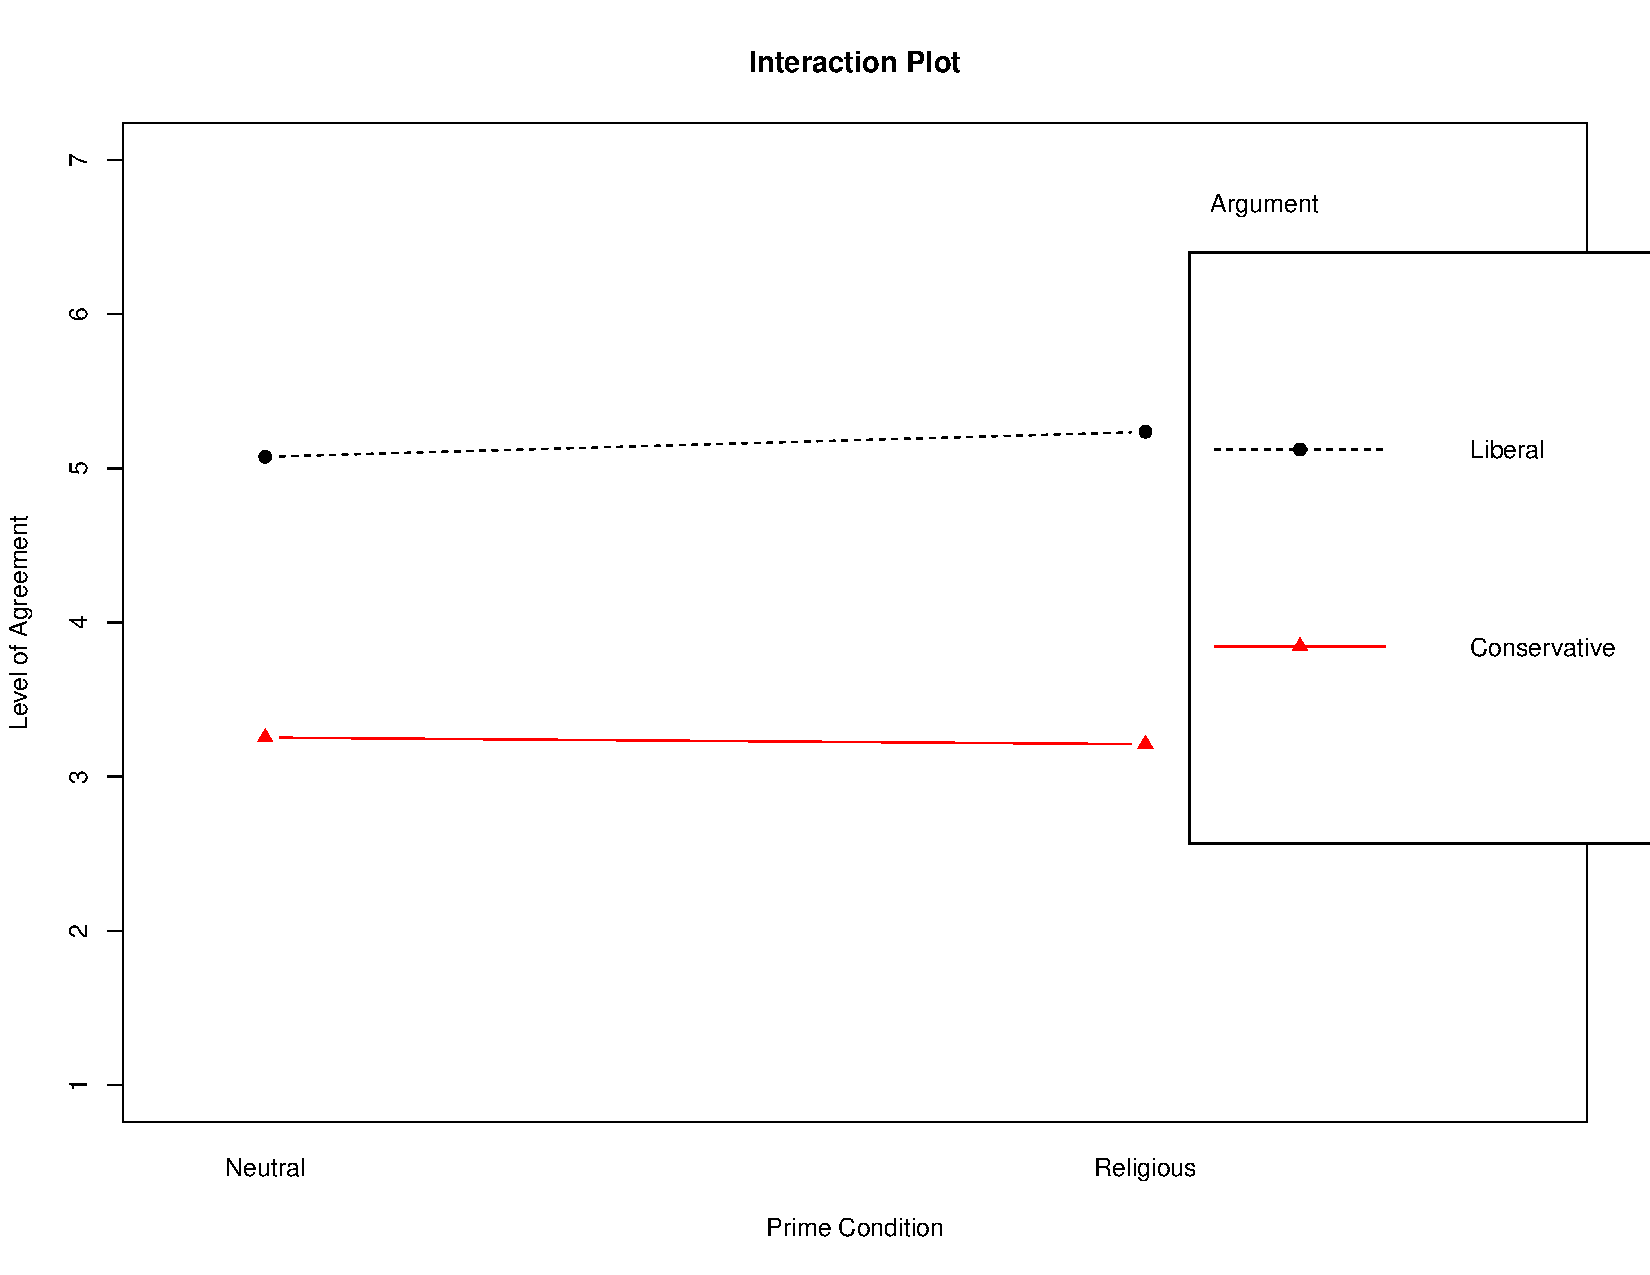
\includegraphics[width=0.8\linewidth]{InteractionPlot}
\captionof{figure}{Figure caption}
\end{center}

Aliquam auctor, metus id ultrices porta, risus enim cursus sapien, quis iaculis sapien tortor sed odio. Mauris ante orci, euismod vitae tincidunt eu, porta ut neque. Aenean sapien est, viverra vel lacinia nec, venenatis eu nulla. Maecenas ut nunc nibh, et tempus libero. Aenean vitae risus ante. Pellentesque condimentum dui. Etiam sagittis purus non tellus tempor volutpat. Donec et dui non massa tristique adipiscing.
\end{multicols}

%------------------------------------------------

\begin{multicols}{2}
\vspace{1em}
Sed fringilla tempus hendrerit. Vestibulum ante ipsum primis in faucibus orci luctus et ultrices posuere cubilia Curae; Etiam ut elit sit amet metus lobortis consequat sit amet in libero. Lorem ipsum dolor sit amet, consectetur adipiscing elit. Phasellus vel sem magna. Nunc at convallis urna. isus ante. Pellentesque condimentum dui. Etiam sagittis purus non tellus tempor volutpat. Donec et dui non massa tristique adipiscing. Quisque vestibulum eros eu.

\begin{center}
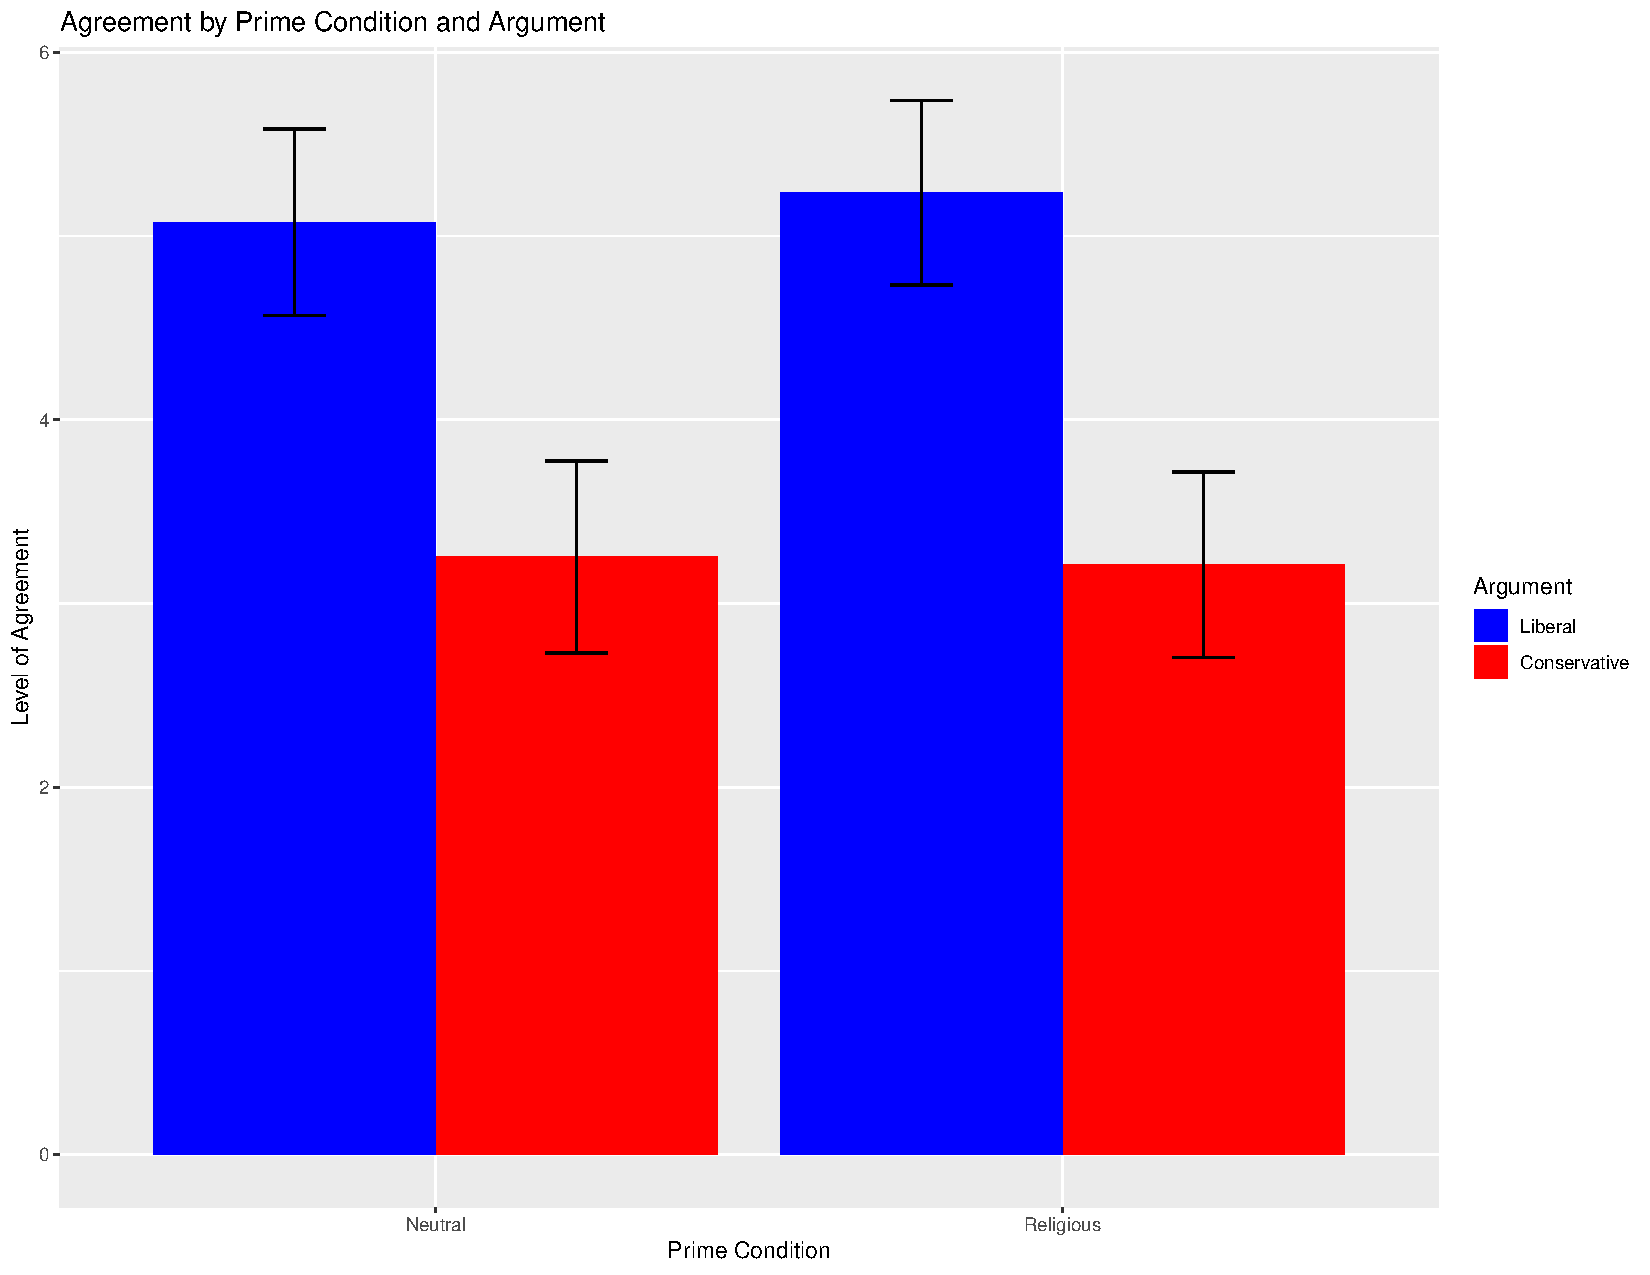
\includegraphics[width=0.8\linewidth]{barplot}
\captionof{figure}{Figure caption}
\end{center}

\end{multicols}
}

%----------------------------------------------------------------------------------------
%	REFERENCES
%----------------------------------------------------------------------------------------

\headerbox{Select Bibliography}{name=references,column=0,above=bottom}{

\renewcommand{\section}[2]{\vskip 0.05em} % Get rid of the default "References" section title
\nocite{*} % Insert publications even if they are not cited in the poster
\footnotesize{ % Reduce the font size in this block
\bibliographystyle{unsrt}
\bibliography{poster} % Use sample.bib as the bibliography file
}}

%----------------------------------------------------------------------------------------
%	FUTURE RESEARCH
%----------------------------------------------------------------------------------------

\headerbox{Future Research}{name=futureresearch,column=1,span=2,aligned=references,above=bottom}{ % This block is as tall as the references block

\begin{multicols}{2}
Integer sed lectus vel mauris euismod suscipit. Praesent a est a est ultricies pellentesque. Donec tincidunt, nunc in feugiat varius, lectus lectus auctor lorem, egestas molestie risus erat ut nibh.

Maecenas viverra ligula a risus blandit vel tincidunt est adipiscing. Suspendisse mollis iaculis sem, in \emph{imperdiet} orci porta vitae. Quisque id dui sed ante sollicitudin sagittis.
\end{multicols}
}

%----------------------------------------------------------------------------------------
%	CONTACT INFORMATION
%----------------------------------------------------------------------------------------

\headerbox{Contact Information}{name=contact,column=3,aligned=references,above=bottom}{ % This block is as tall as the references block

\begin{description}\compresslist
\item[Web] www.ncf.edu
\item[Email] jennifer.lin16@ncf.edu|sgraham@ncf.edu
\item[Phone] +1 (941) 487 5000
\end{description}
}

%----------------------------------------------------------------------------------------
%	CONCLUSION
%----------------------------------------------------------------------------------------

\headerbox{Conclusion}{name=conclusion,column=2,span=2,row=0,below=results,above=references}{

\begin{multicols}{2}

\tikzstyle{decision} = [diamond, draw, fill=blue!20, text width=4.5em, text badly centered, node distance=2cm, inner sep=0pt]
\tikzstyle{block} = [rectangle, draw, fill=blue!20, text width=5em, text centered, rounded corners, minimum height=4em]
\tikzstyle{line} = [draw, -latex']
\tikzstyle{cloud} = [draw, ellipse, fill=red!20, node distance=3cm, minimum height=2em]

\begin{tikzpicture}[node distance = 2cm, auto]
\node [block] (init) {Initialize Model};
\node [cloud, left of=init] (Start) {Start};
\node [cloud, right of=init] (Start2) {Start Two};
\node [block, below of=init] (init2) {Initialize Two};
\node [decision, below of=init2] (End) {End};
\path [line] (init) -- (init2);
\path [line] (init2) -- (End);
\path [line, dashed] (Start) -- (init);
\path [line, dashed] (Start2) -- (init);
\path [line, dashed] (Start2) |- (init2);
\end{tikzpicture}

%------------------------------------------------

\begin{itemize}\compresslist
\item Pellentesque eget orci eros. Fusce ultricies, tellus et pellentesque fringilla, ante massa luctus libero, quis tristique purus urna nec nibh. Phasellus fermentum rutrum elementum. Nam quis justo lectus.
\item Vestibulum sem ante, hendrerit a gravida ac, blandit quis magna.
\item Donec sem metus, facilisis at condimentum eget, vehicula ut massa. Morbi consequat, diam sed convallis tincidunt, arcu nunc.
\item Nunc at convallis urna. isus ante. Pellentesque condimentum dui. Etiam sagittis purus non tellus tempor volutpat. Donec et dui non massa tristique adipiscing.
\end{itemize}

\end{multicols}
}

%----------------------------------------------------------------------------------------
%	MATERIALS AND METHODS
%----------------------------------------------------------------------------------------

\headerbox{Previous Research}{name=method,column=0,below=objectives,bottomaligned=conclusion}{ % This block's bottom aligns with the bottom of the conclusion block



Americans are religious individuals, with 85\% of people identifying with a major denomination of worship. As such, religion becomes a part of identity that can influence political decisions. Since religions teach people about living moral lives, this world view can be applied to understanding how politics ought to be. Voting in churches can serve as reminders to people's faiths and subliminally prime their political stances.
}

%----------------------------------------------------------------------------------------
%	RESULTS 2
%----------------------------------------------------------------------------------------

\headerbox{Materials \& Methods}{name=results2,column=1,below=objectives,bottomaligned=conclusion}{ % This block's bottom aligns with the bottom of the conclusion block

The Participants for the study were as follows: 
\begin{itemize} \compresslist
	\item 304 of 356 original respondents incorporated in analysis (126 identify as female)
	\item Recruited via Amazon Mechanical Turk
	\item Participants were paid \$1 for their participation
\end{itemize}

The tasks each participant completed are:

\begin{itemize} \compresslist
	\item \tb{Sentence Reorganization} -- Participants saw 5 word chunks (of religious or neutral content) and had to rearrange them to make logical sentences.
	\item \tb{Statement and Agreement on Controversial Issue} -- Participants read vignettes supporting or countering abortion and were asked to rate the quality of the argument along with the extent they agreed
	\item \tb{Religiosity Measure} -- Survey on religious identity
	\item \tb{Demographic Questions} -- Questions include race, gender, and political affiliation 
	\item \tb{Manipulation Check}
\end{itemize}
}

%----------------------------------------------------------------------------------------

\end{poster}

\end{document}